\documentclass[]{article}
\usepackage{lmodern}
\usepackage{amssymb,amsmath}
\usepackage{ifxetex,ifluatex}
\usepackage{fixltx2e} % provides \textsubscript
\ifnum 0\ifxetex 1\fi\ifluatex 1\fi=0 % if pdftex
  \usepackage[T1]{fontenc}
  \usepackage[utf8]{inputenc}
\else % if luatex or xelatex
  \ifxetex
    \usepackage{mathspec}
  \else
    \usepackage{fontspec}
  \fi
  \defaultfontfeatures{Ligatures=TeX,Scale=MatchLowercase}
\fi
% use upquote if available, for straight quotes in verbatim environments
\IfFileExists{upquote.sty}{\usepackage{upquote}}{}
% use microtype if available
\IfFileExists{microtype.sty}{%
\usepackage{microtype}
\UseMicrotypeSet[protrusion]{basicmath} % disable protrusion for tt fonts
}{}
\usepackage[margin=1in]{geometry}
\usepackage{hyperref}
\hypersetup{unicode=true,
            pdftitle={Analysis of Teaching Evaluations},
            pdfauthor={Dave Bridges},
            pdfborder={0 0 0},
            breaklinks=true}
\urlstyle{same}  % don't use monospace font for urls
\usepackage{color}
\usepackage{fancyvrb}
\newcommand{\VerbBar}{|}
\newcommand{\VERB}{\Verb[commandchars=\\\{\}]}
\DefineVerbatimEnvironment{Highlighting}{Verbatim}{commandchars=\\\{\}}
% Add ',fontsize=\small' for more characters per line
\usepackage{framed}
\definecolor{shadecolor}{RGB}{248,248,248}
\newenvironment{Shaded}{\begin{snugshade}}{\end{snugshade}}
\newcommand{\KeywordTok}[1]{\textcolor[rgb]{0.13,0.29,0.53}{\textbf{{#1}}}}
\newcommand{\DataTypeTok}[1]{\textcolor[rgb]{0.13,0.29,0.53}{{#1}}}
\newcommand{\DecValTok}[1]{\textcolor[rgb]{0.00,0.00,0.81}{{#1}}}
\newcommand{\BaseNTok}[1]{\textcolor[rgb]{0.00,0.00,0.81}{{#1}}}
\newcommand{\FloatTok}[1]{\textcolor[rgb]{0.00,0.00,0.81}{{#1}}}
\newcommand{\ConstantTok}[1]{\textcolor[rgb]{0.00,0.00,0.00}{{#1}}}
\newcommand{\CharTok}[1]{\textcolor[rgb]{0.31,0.60,0.02}{{#1}}}
\newcommand{\SpecialCharTok}[1]{\textcolor[rgb]{0.00,0.00,0.00}{{#1}}}
\newcommand{\StringTok}[1]{\textcolor[rgb]{0.31,0.60,0.02}{{#1}}}
\newcommand{\VerbatimStringTok}[1]{\textcolor[rgb]{0.31,0.60,0.02}{{#1}}}
\newcommand{\SpecialStringTok}[1]{\textcolor[rgb]{0.31,0.60,0.02}{{#1}}}
\newcommand{\ImportTok}[1]{{#1}}
\newcommand{\CommentTok}[1]{\textcolor[rgb]{0.56,0.35,0.01}{\textit{{#1}}}}
\newcommand{\DocumentationTok}[1]{\textcolor[rgb]{0.56,0.35,0.01}{\textbf{\textit{{#1}}}}}
\newcommand{\AnnotationTok}[1]{\textcolor[rgb]{0.56,0.35,0.01}{\textbf{\textit{{#1}}}}}
\newcommand{\CommentVarTok}[1]{\textcolor[rgb]{0.56,0.35,0.01}{\textbf{\textit{{#1}}}}}
\newcommand{\OtherTok}[1]{\textcolor[rgb]{0.56,0.35,0.01}{{#1}}}
\newcommand{\FunctionTok}[1]{\textcolor[rgb]{0.00,0.00,0.00}{{#1}}}
\newcommand{\VariableTok}[1]{\textcolor[rgb]{0.00,0.00,0.00}{{#1}}}
\newcommand{\ControlFlowTok}[1]{\textcolor[rgb]{0.13,0.29,0.53}{\textbf{{#1}}}}
\newcommand{\OperatorTok}[1]{\textcolor[rgb]{0.81,0.36,0.00}{\textbf{{#1}}}}
\newcommand{\BuiltInTok}[1]{{#1}}
\newcommand{\ExtensionTok}[1]{{#1}}
\newcommand{\PreprocessorTok}[1]{\textcolor[rgb]{0.56,0.35,0.01}{\textit{{#1}}}}
\newcommand{\AttributeTok}[1]{\textcolor[rgb]{0.77,0.63,0.00}{{#1}}}
\newcommand{\RegionMarkerTok}[1]{{#1}}
\newcommand{\InformationTok}[1]{\textcolor[rgb]{0.56,0.35,0.01}{\textbf{\textit{{#1}}}}}
\newcommand{\WarningTok}[1]{\textcolor[rgb]{0.56,0.35,0.01}{\textbf{\textit{{#1}}}}}
\newcommand{\AlertTok}[1]{\textcolor[rgb]{0.94,0.16,0.16}{{#1}}}
\newcommand{\ErrorTok}[1]{\textcolor[rgb]{0.64,0.00,0.00}{\textbf{{#1}}}}
\newcommand{\NormalTok}[1]{{#1}}
\usepackage{graphicx,grffile}
\makeatletter
\def\maxwidth{\ifdim\Gin@nat@width>\linewidth\linewidth\else\Gin@nat@width\fi}
\def\maxheight{\ifdim\Gin@nat@height>\textheight\textheight\else\Gin@nat@height\fi}
\makeatother
% Scale images if necessary, so that they will not overflow the page
% margins by default, and it is still possible to overwrite the defaults
% using explicit options in \includegraphics[width, height, ...]{}
\setkeys{Gin}{width=\maxwidth,height=\maxheight,keepaspectratio}
\IfFileExists{parskip.sty}{%
\usepackage{parskip}
}{% else
\setlength{\parindent}{0pt}
\setlength{\parskip}{6pt plus 2pt minus 1pt}
}
\setlength{\emergencystretch}{3em}  % prevent overfull lines
\providecommand{\tightlist}{%
  \setlength{\itemsep}{0pt}\setlength{\parskip}{0pt}}
\setcounter{secnumdepth}{0}
% Redefines (sub)paragraphs to behave more like sections
\ifx\paragraph\undefined\else
\let\oldparagraph\paragraph
\renewcommand{\paragraph}[1]{\oldparagraph{#1}\mbox{}}
\fi
\ifx\subparagraph\undefined\else
\let\oldsubparagraph\subparagraph
\renewcommand{\subparagraph}[1]{\oldsubparagraph{#1}\mbox{}}
\fi

%%% Use protect on footnotes to avoid problems with footnotes in titles
\let\rmarkdownfootnote\footnote%
\def\footnote{\protect\rmarkdownfootnote}

%%% Change title format to be more compact
\usepackage{titling}

% Create subtitle command for use in maketitle
\newcommand{\subtitle}[1]{
  \posttitle{
    \begin{center}\large#1\end{center}
    }
}

\setlength{\droptitle}{-2em}
  \title{Analysis of Teaching Evaluations}
  \pretitle{\vspace{\droptitle}\centering\huge}
  \posttitle{\par}
  \author{Dave Bridges}
  \preauthor{\centering\large\emph}
  \postauthor{\par}
  \predate{\centering\large\emph}
  \postdate{\par}
  \date{1/28/2018}


\begin{document}
\maketitle

{
\setcounter{tocdepth}{2}
\tableofcontents
}
\subsection{Data Import}\label{data-import}

Copied evaluation table, added quotes around the questions and imported
into excel. Converted this to a csv file for import. Did this for both
2016 and 2017 teaching evaluations, downloaded from wolverine access.

\begin{Shaded}
\begin{Highlighting}[]
\KeywordTok{library}\NormalTok{(readr)}
\KeywordTok{library}\NormalTok{(dplyr)}
\NormalTok{data}\FloatTok{.2016}\NormalTok{.datafile <-}\StringTok{ '2016 Evaluations.csv'}
\NormalTok{data}\FloatTok{.2017}\NormalTok{.datafile <-}\StringTok{ '2017 Evaluations.csv'}

\NormalTok{input_col_types <-}\StringTok{ }\KeywordTok{cols}\NormalTok{(}
  \DataTypeTok{Number =} \KeywordTok{col_factor}\NormalTok{(}\DataTypeTok{levels=}\OtherTok{NULL}\NormalTok{),}
  \DataTypeTok{Question =} \KeywordTok{col_factor}\NormalTok{(}\DataTypeTok{levels=}\OtherTok{NULL}\NormalTok{))}

\NormalTok{data}\FloatTok{.2016} \NormalTok{<-}\StringTok{ }\KeywordTok{read_csv}\NormalTok{(data}\FloatTok{.2016}\NormalTok{.datafile, }\DataTypeTok{col_types=}\NormalTok{input_col_types) %>%}\StringTok{ }\KeywordTok{mutate}\NormalTok{(}\DataTypeTok{Year=}\StringTok{"2016"}\NormalTok{)}
\NormalTok{data}\FloatTok{.2017} \NormalTok{<-}\StringTok{ }\KeywordTok{read_csv}\NormalTok{(data}\FloatTok{.2017}\NormalTok{.datafile, }\DataTypeTok{col_types=}\NormalTok{input_col_types)  %>%}\StringTok{ }\KeywordTok{mutate}\NormalTok{(}\DataTypeTok{Year=}\StringTok{"2017"}\NormalTok{)}

\NormalTok{te.data.wide <-}\StringTok{ }\KeywordTok{full_join}\NormalTok{(data}\FloatTok{.2016}\NormalTok{,data}\FloatTok{.2017}\NormalTok{, }
                     \DataTypeTok{by =} \KeywordTok{c}\NormalTok{(}\StringTok{"Number"}\NormalTok{, }\StringTok{"Question"}\NormalTok{), }
                     \DataTypeTok{suffix =} \KeywordTok{c}\NormalTok{(}\StringTok{".16"}\NormalTok{, }\StringTok{".17"}\NormalTok{))}

\NormalTok{te.data <-}\StringTok{ }
\StringTok{  }\KeywordTok{rbind}\NormalTok{(data}\FloatTok{.2016}\NormalTok{,data}\FloatTok{.2017}\NormalTok{) %>%}
\StringTok{  }\KeywordTok{mutate}\NormalTok{(}\DataTypeTok{Total =} \NormalTok{SD+D+N+A+SA) %>%}
\StringTok{  }\KeywordTok{mutate}\NormalTok{(}\StringTok{`}\DataTypeTok{Strongly Disagree}\StringTok{`}\NormalTok{=SD/Total*}\DecValTok{100}\NormalTok{,}
         \StringTok{`}\DataTypeTok{Disagree}\StringTok{`}\NormalTok{=D/Total*}\DecValTok{100}\NormalTok{,}
         \StringTok{`}\DataTypeTok{Neutral}\StringTok{`}\NormalTok{=N/Total*}\DecValTok{100}\NormalTok{,}
         \StringTok{`}\DataTypeTok{Agree}\StringTok{`}\NormalTok{=A/Total*}\DecValTok{100}\NormalTok{,}
         \StringTok{`}\DataTypeTok{Strongly Agree}\StringTok{`}\NormalTok{=SA/Total*}\DecValTok{100}\NormalTok{)}
\end{Highlighting}
\end{Shaded}

The imported datafiles include:

\begin{itemize}
\tightlist
\item
  2016 Evaluations.csv
\item
  2017 Evaluations.csv
\end{itemize}

\section{Overall Questions}\label{overall-questions}

\subsection{Overall, this was an excellent
course.}\label{overall-this-was-an-excellent-course.}

\begin{Shaded}
\begin{Highlighting}[]
\NormalTok{overall.data <-}
\StringTok{  }\NormalTok{te.data %>%}
\StringTok{  }\KeywordTok{filter}\NormalTok{(Number==}\DecValTok{1}\NormalTok{) %>%}
\StringTok{  }\KeywordTok{mutate}\NormalTok{(}\DataTypeTok{Item=}\KeywordTok{as.factor}\NormalTok{(Year))}

\KeywordTok{library}\NormalTok{(HH)}

\NormalTok{plot.data <-}\StringTok{ }\NormalTok{overall.data[}\DecValTok{7}\NormalTok{:}\DecValTok{3}\NormalTok{]}
\KeywordTok{rownames}\NormalTok{(plot.data) <-}\StringTok{ }\KeywordTok{c}\NormalTok{(}\StringTok{"Before"}\NormalTok{,}\StringTok{"After"}\NormalTok{)}

\KeywordTok{likert}\NormalTok{(plot.data, }\DataTypeTok{horizontal =} \OtherTok{FALSE}\NormalTok{,}
       \DataTypeTok{main =} \StringTok{"Overall, this was an excellent course."}\NormalTok{,}
       \DataTypeTok{xlab =} \StringTok{"Percent"}\NormalTok{, }\CommentTok{# becomes ylab due to horizontal arg,}
       \DataTypeTok{ylab =} \KeywordTok{c}\NormalTok{(}\StringTok{"Before"}\NormalTok{,}\StringTok{"After"}\NormalTok{),}
       \DataTypeTok{title =} \StringTok{"Overall, this was an excellent course."}\NormalTok{,}
       \DataTypeTok{auto.key =} \KeywordTok{list}\NormalTok{(}\DataTypeTok{space =} \StringTok{"right"}\NormalTok{, }\DataTypeTok{columns =} \DecValTok{1}\NormalTok{,}
                     \DataTypeTok{reverse =} \OtherTok{TRUE}\NormalTok{))}
\end{Highlighting}
\end{Shaded}

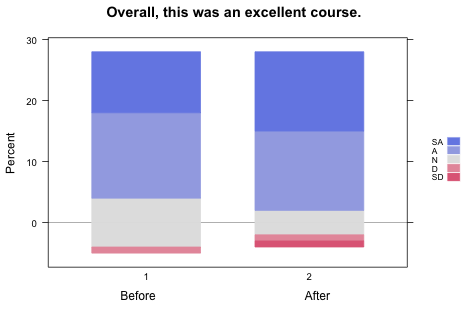
\includegraphics{figures/excellent-course-1.png}

\subsection{This course advanced my understanding of the subject
matter.}\label{this-course-advanced-my-understanding-of-the-subject-matter.}

\begin{Shaded}
\begin{Highlighting}[]
\NormalTok{overall.data <-}
\StringTok{  }\NormalTok{te.data %>%}
\StringTok{  }\KeywordTok{filter}\NormalTok{(Number==}\DecValTok{1631}\NormalTok{) %>%}
\StringTok{  }\KeywordTok{mutate}\NormalTok{(}\DataTypeTok{Item=}\KeywordTok{as.factor}\NormalTok{(Year))}

\NormalTok{plot.data <-}\StringTok{ }\NormalTok{overall.data[}\DecValTok{7}\NormalTok{:}\DecValTok{3}\NormalTok{]}
\KeywordTok{rownames}\NormalTok{(plot.data) <-}\StringTok{ }\KeywordTok{c}\NormalTok{(}\StringTok{"Before"}\NormalTok{,}\StringTok{"After"}\NormalTok{)}

\KeywordTok{likert}\NormalTok{(plot.data, }\DataTypeTok{horizontal =} \OtherTok{FALSE}\NormalTok{,}
       \DataTypeTok{main =} \StringTok{"This course advanced my understanding of the subject matter."}\NormalTok{,}
       \DataTypeTok{xlab =} \StringTok{"Percent"}\NormalTok{, }\CommentTok{# becomes ylab due to horizontal arg,}
       \DataTypeTok{ylab =} \KeywordTok{c}\NormalTok{(}\StringTok{"Before"}\NormalTok{,}\StringTok{"After"}\NormalTok{),}
       \DataTypeTok{title =} \StringTok{"Overall, this was an excellent course."}\NormalTok{,}
       \DataTypeTok{auto.key =} \KeywordTok{list}\NormalTok{(}\DataTypeTok{space =} \StringTok{"right"}\NormalTok{, }\DataTypeTok{columns =} \DecValTok{1}\NormalTok{,}
                     \DataTypeTok{reverse =} \OtherTok{TRUE}\NormalTok{))}
\end{Highlighting}
\end{Shaded}

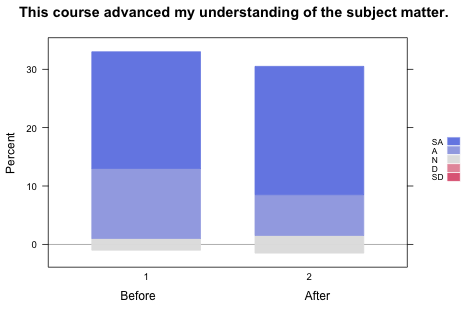
\includegraphics{figures/advanced-understanding-1.png}

\subsection{I learned a great deal from this
course.}\label{i-learned-a-great-deal-from-this-course.}

\begin{Shaded}
\begin{Highlighting}[]
\NormalTok{overall.data <-}
\StringTok{  }\NormalTok{te.data %>%}
\StringTok{  }\KeywordTok{filter}\NormalTok{(Number==}\DecValTok{3}\NormalTok{) %>%}
\StringTok{  }\KeywordTok{mutate}\NormalTok{(}\DataTypeTok{Item=}\KeywordTok{as.factor}\NormalTok{(Year))}

\NormalTok{plot.data <-}\StringTok{ }\NormalTok{overall.data[}\DecValTok{7}\NormalTok{:}\DecValTok{3}\NormalTok{]}
\KeywordTok{rownames}\NormalTok{(plot.data) <-}\StringTok{ }\KeywordTok{c}\NormalTok{(}\StringTok{"Before"}\NormalTok{,}\StringTok{"After"}\NormalTok{)}

\KeywordTok{likert}\NormalTok{(plot.data, }\DataTypeTok{horizontal =} \OtherTok{FALSE}\NormalTok{,}
       \DataTypeTok{main =} \StringTok{"I learned a great deal from this course."}\NormalTok{,}
       \DataTypeTok{xlab =} \StringTok{"Percent"}\NormalTok{, }\CommentTok{# becomes ylab due to horizontal arg,}
       \DataTypeTok{ylab =} \KeywordTok{c}\NormalTok{(}\StringTok{"Before"}\NormalTok{,}\StringTok{"After"}\NormalTok{),}
       \DataTypeTok{auto.key =} \KeywordTok{list}\NormalTok{(}\DataTypeTok{space =} \StringTok{"right"}\NormalTok{, }\DataTypeTok{columns =} \DecValTok{1}\NormalTok{,}
                     \DataTypeTok{reverse =} \OtherTok{TRUE}\NormalTok{))}
\end{Highlighting}
\end{Shaded}

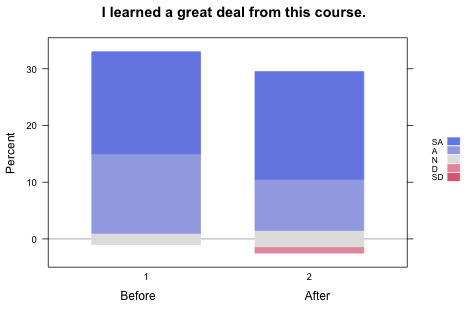
\includegraphics{figures/learned-great-deal-1.png}

\section{The grades in this course were fairly
determined.}\label{the-grades-in-this-course-were-fairly-determined.}

\begin{Shaded}
\begin{Highlighting}[]
\NormalTok{overall.data <-}
\StringTok{  }\NormalTok{te.data %>%}
\StringTok{  }\KeywordTok{filter}\NormalTok{(Number==}\DecValTok{894}\NormalTok{) %>%}
\StringTok{  }\KeywordTok{mutate}\NormalTok{(}\DataTypeTok{Item=}\KeywordTok{as.factor}\NormalTok{(Year))}

\NormalTok{plot.data <-}\StringTok{ }\NormalTok{overall.data[}\DecValTok{7}\NormalTok{:}\DecValTok{3}\NormalTok{]}
\KeywordTok{rownames}\NormalTok{(plot.data) <-}\StringTok{ }\KeywordTok{c}\NormalTok{(}\StringTok{"Before"}\NormalTok{,}\StringTok{"After"}\NormalTok{)}

\KeywordTok{likert}\NormalTok{(plot.data, }\DataTypeTok{horizontal =} \OtherTok{FALSE}\NormalTok{,}
       \DataTypeTok{main =} \StringTok{"The grades in this course were fairly determined."}\NormalTok{, }\CommentTok{# or give "title",}
       \DataTypeTok{xlab =} \StringTok{"Percent"}\NormalTok{, }\CommentTok{# becomes ylab due to horizontal arg,}
       \DataTypeTok{ylab =} \KeywordTok{c}\NormalTok{(}\StringTok{"Before"}\NormalTok{,}\StringTok{"After"}\NormalTok{),}
       \DataTypeTok{title =} \StringTok{"Overall, this was an excellent course."}\NormalTok{,}
       \DataTypeTok{auto.key =} \KeywordTok{list}\NormalTok{(}\DataTypeTok{space =} \StringTok{"right"}\NormalTok{, }\DataTypeTok{columns =} \DecValTok{1}\NormalTok{,}
                     \DataTypeTok{reverse =} \OtherTok{TRUE}\NormalTok{))}
\end{Highlighting}
\end{Shaded}

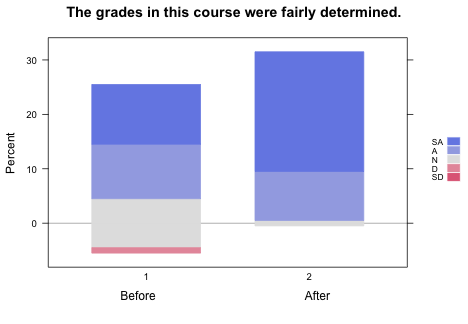
\includegraphics{figures/grades-fairly-determined-1.png}


\end{document}
